\documentclass[a4paper,10pt]{report}
\usepackage[utf8x]{inputenc}
\usepackage[T1]{fontenc}
\usepackage[french]{babel} 
\usepackage{lmodern} % Pour changer le pack de police
\usepackage{makeidx}
\usepackage{graphicx}
\graphicspath{{figures/}}
\usepackage[margin=3cm]{geometry}
\usepackage{array}
\usepackage{float}
%\usepackage[cc]{titlepic}
\usepackage{amsmath}

%\titlepic{
%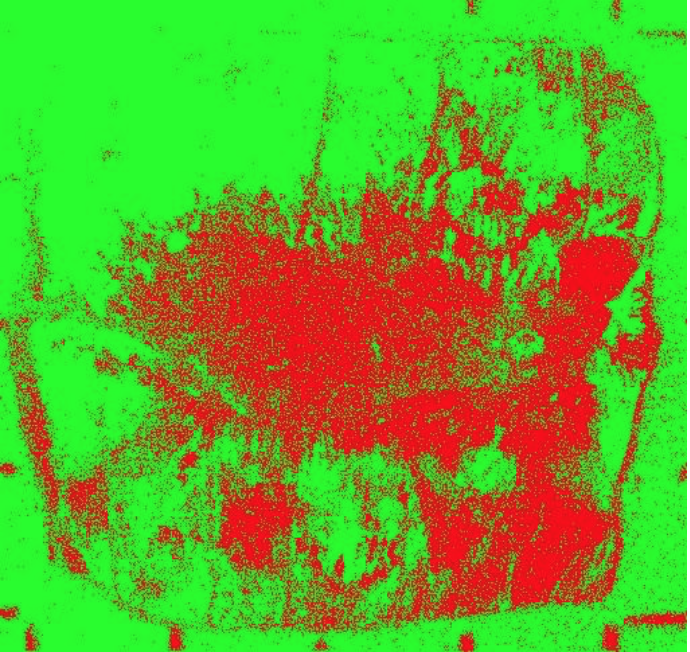
\includegraphics[width=7cm]{titlepic1.png}
%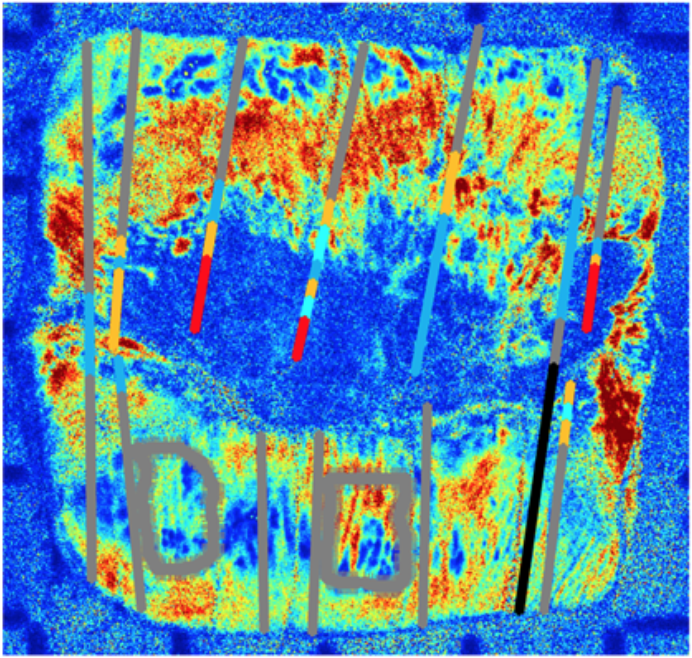
\includegraphics[width=7cm]{titlepic2.png}
%}
\title{Projet 3A\\Analyse d'imagerie polarimétrique}
\author{\textsc{Guinaudeau} Alexandre\\
	\and 
	\textsc{Hulot} Pierre
	\and 
	\textsc{Dejoie} Etienne	
	}
\date{\today}
\makeindex 
\begin{document}

\maketitle
\chapter*{Remerciements}
Nous tenons à remercier toute l'équipe d'ADM Polar qui nous a fait confiance pour mener ce projet. Ils ont su prendre le temps de nous expliquer les enjeux de l'analyse de données pour ADM Polar. Ils nous ont également fourni un ensemble de données nous permettant de mettre en application des techniques d'apprentissage et ainsi de mieux les comprendre.
Un grand remerciement également aux développeurs de la bibliothèque scikit sur laquelle nous nous sommes largement appuyés tout au long de ce projet.

\chapter*{Introduction}

Aujourd'hui, le dépistage du cancer du col de l'utérus est effectué à l'\oe il nu. Si la patiente est effectivement atteinte d'un cancer, un échantillon (appelé conisation) est prélevé, et un spécialiste découpe l'échantillon pour déterminer les zones atteintes. \emph{ADM polar} cherche à détecter les cellules cancéreuses à partir d'imagerie polarimétrique. 
L'idée à terme serait de concevoir un outil qui permette de détecter les zones effectivement atteintes \emph{in vivo}, pour ainsi mieux délimiter la zone à prélever et réduire les risques de prélèvement pour les patientes saines.

\emph{ADM polar} fait analyser ces échantillons par un spécialiste, pour déterminer l'état (sain, malade, bénin...) des cellules le long de coupes.
Puis, après avoir pris plusieurs images dans des configurations de polarisation différentes, \emph{ADM polar} reconstitue la matrice de Müller de l'échantillon, un ensemble de 16 images qui représentent l'état de polarisation.
Il reste alors à déterminer la corrélation entre les valeurs dans la matrice de Müller d'une cellule et son diagnostic.

Dans le cadre du projet de 3e année, nous avons souhaité appliquer les connaissances théoriques apprises en cours à des données réelles. Nous avons donc rejoint le projet d'\emph{ADM polar}, dans le but de détecter les cellules cancéreuses, à partir des images polarimétriques fournies par \emph{ADM polar}.

La première étape a été la visualisation des données, pour mieux savoir quels modèles d'apprentissage seraient les plus susceptibles de porter leurs fruits. Puis, nous avons cherché à réduire la dimension du problème en sélectionnant les paramètres les plus discriminants dans la classification des cellules. Enfin, nous avons testé différents modèles de classification et mesuré leurs performances en termes de précision et de coût de calcul.
\chapter{Contexte}

\vspace*{-12pt} %Sinon la dernière ligne du chapitre dépasse

\section{ADM Polar, contexte du projet}
Le principal partenaire du projet est ADM Polar, une start-up d'imagerie médicale basée sur la collecte et l'analyse de données polarimétriques. L'objectif de la start-up est d'utiliser ces données afin de diagnostiquer de façon automatisée des cellules cancéreuses (et en particulier le cancer col de l'uterus). Une première étude \emph{in vivo} menée sur 140 patientes leur a fourni une large base de données sur laquelle ils comptent construire leur entreprise grâce à de l'analyse Big Data. Lors d'un événement du Cabinet Start-up, organisé par les élèves de l'École polytechnique, nous les avons rencontrés une première fois. Les membres de la start-up nous ont alors expliqué qu'ils avaient énormément de données à valoriser mais qu'ils ne savaient pas comment faire (leur domaine respectif étant plutôt relié à la physique et au médical). Nous avons donc décidé, dans le cadre du projet 3A, de nous lancer dans cette entreprise ambitieuse, à l'aide de nos connaissances en informatique et de nos cours de Big Data. La start-up étant localisée dans les laboratoires de l'école, les rencontres, échanges et suivis étaient simplifiés, tout au long du projet.
\section{Présentation des données}
Pour ce projet, nous disposions d'un jeu de données de $163 000$ pixels répartis sur 17 images différentes. Pour chaque pixel, nous avions les 16 éléments de la matrice de Müller, leur position, leur diagnostic, et l'image correspondante.
Ces pixels sont répartis en $4/5$ de sains et $1/5$ de malades. L'affichage des pixels nous montre que pour chaque image, les pixels sont répartis en zones au diagnostic identique. Sur les $17$ images, $11$ ne possèdent que des zones saines, une a une zone saine et une zone malade et les $5$ dernières n’ont que des zones malades. Le nombre d'images étant assez limité, il n'a pas été facile de discriminer les pixels sains des pixels malades.

\begin{figure}[htbp]
  \caption{Répartition des zones}
  \centering
  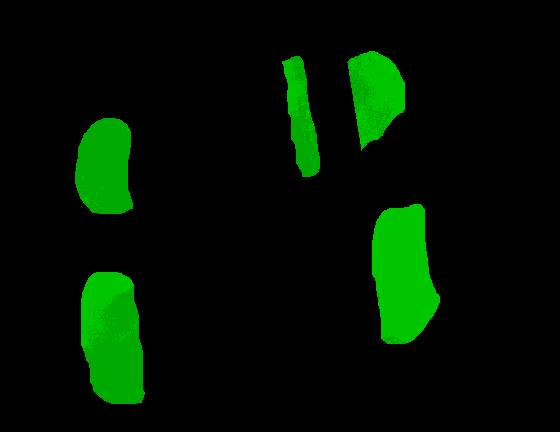
\includegraphics[width=3cm]{piece(1).jpg}
  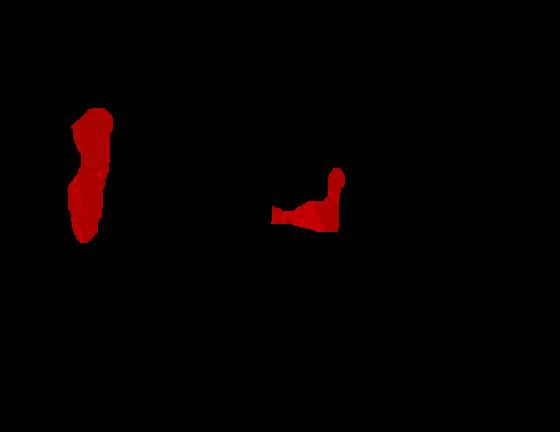
\includegraphics[width=3cm]{piece(2).jpg}
  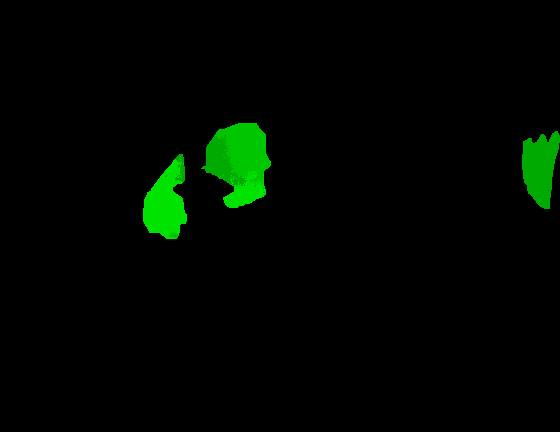
\includegraphics[width=3cm]{piece(3).jpg}
  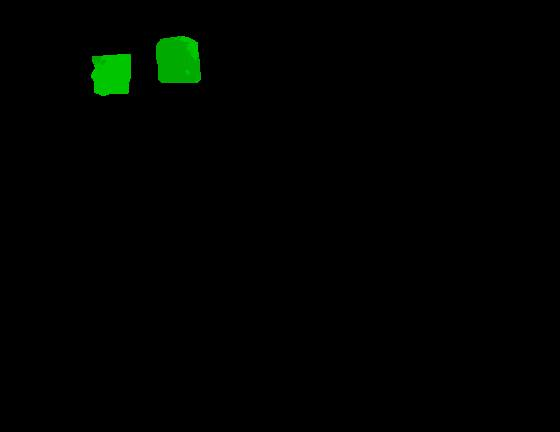
\includegraphics[width=3cm]{piece(4).jpg}
  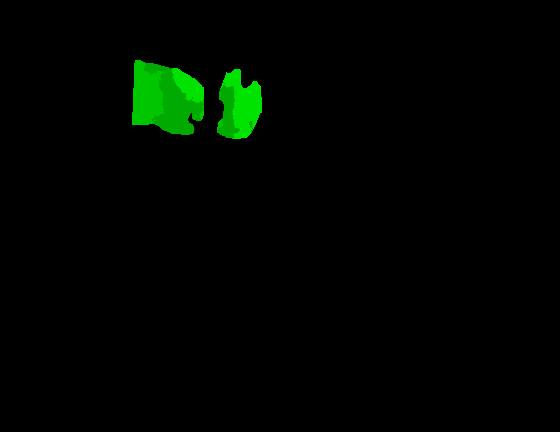
\includegraphics[width=3cm]{piece(5).jpg}
  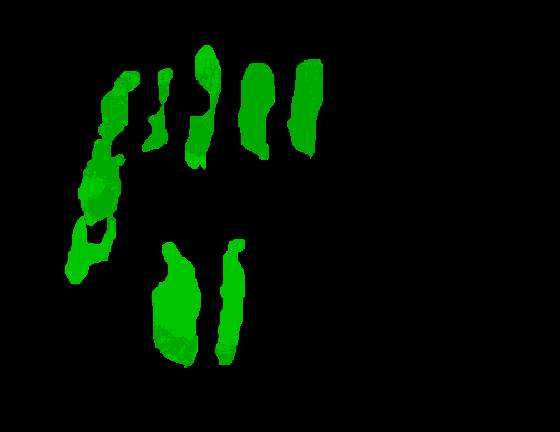
\includegraphics[width=3cm]{piece(6).jpg}
  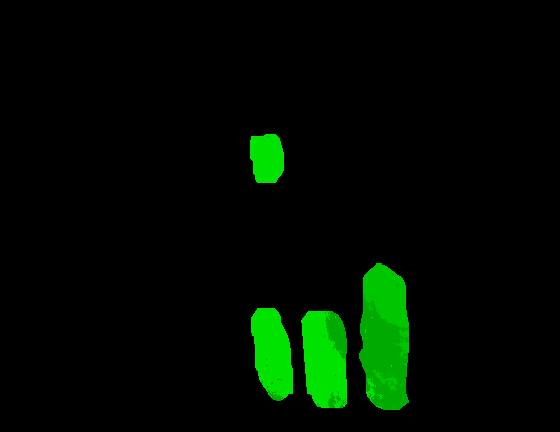
\includegraphics[width=3cm]{piece(7).jpg}
  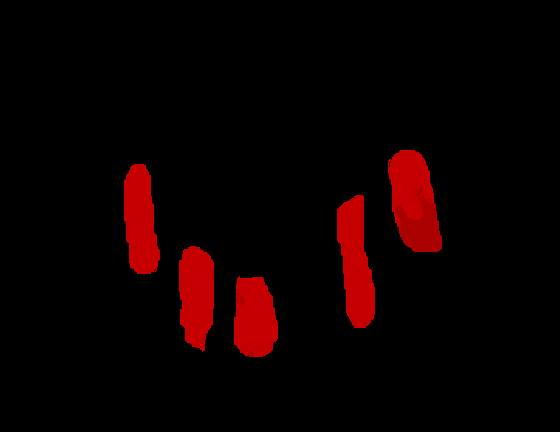
\includegraphics[width=3cm]{piece(8).jpg}
  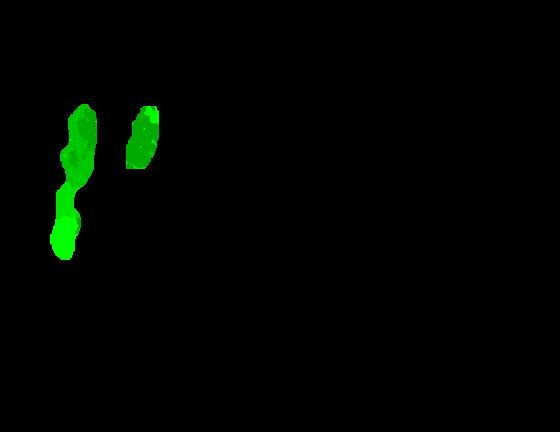
\includegraphics[width=3cm]{piece(9).jpg}
  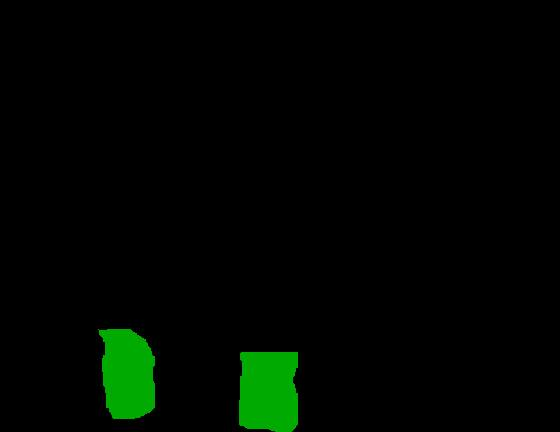
\includegraphics[width=3cm]{piece(10).jpg}
  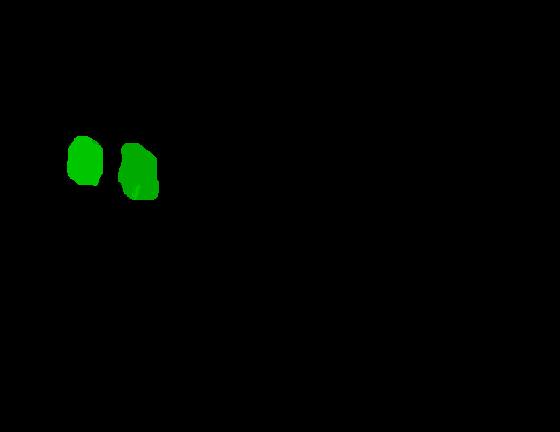
\includegraphics[width=3cm]{piece(11).jpg}
  
\includegraphics[width=3cm]{piece(12).jpg}
  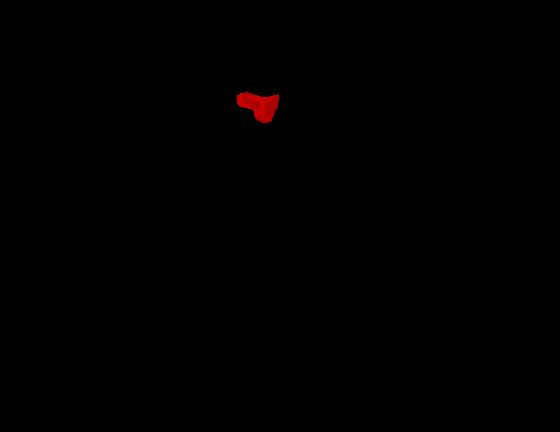
\includegraphics[width=3cm]{piece(13).jpg}
  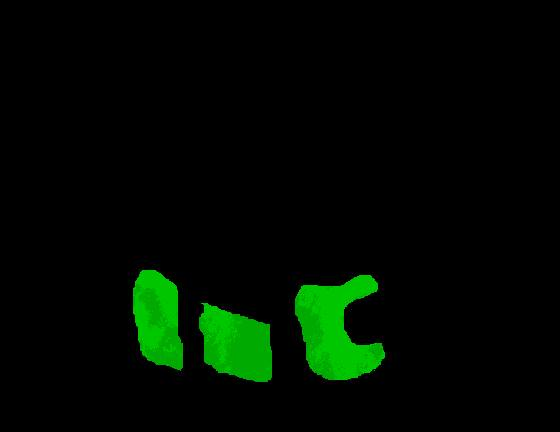
\includegraphics[width=3cm]{piece(14).jpg}
  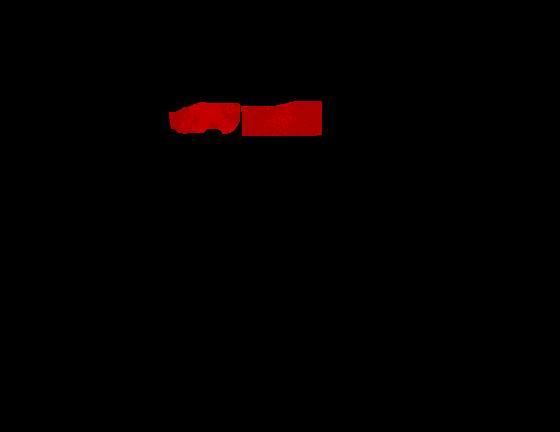
\includegraphics[width=3cm]{piece(15).jpg}
  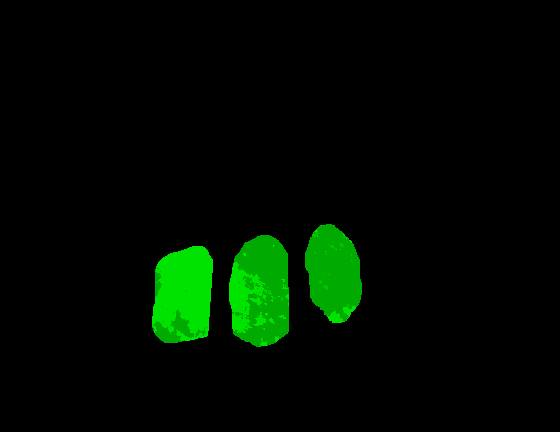
\includegraphics[width=3cm]{piece(16).jpg}
  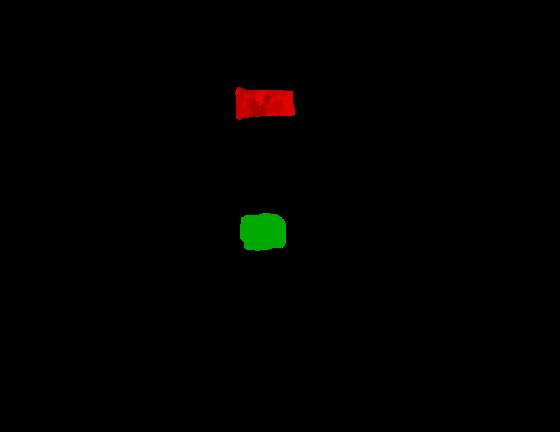
\includegraphics[width=3cm]{piece(17).jpg}
\end{figure}

\subsection{la Matrice de Müller}
\index{Matrice de Müller}
Les données sont obtenues par polarisation de la lumière. De la lumière polarisée est envoyée sur l'échantillon, réfléchie par celui-ci, puis analysée.
La matrice de Müller est obtenue à partir de l'analyse de la polarisation de la lumière réfléchie. Le postulat du laboratoire sur lequel repose tout le traitement des données est que les cellules saines et malades polarisent différemment la lumière. Cela implique qu'il est possible de reconnaître une cellule malade par la polarisation de la lumière réfléchie.
Le PICM se base pour cela sur l’observation de relations entre les images polarisées et le diagnostic correspondant. 
La polarisation génère 16 images par échantillon. On associe alors à chaque pixel une matrice $4x4$ appelée matrice de Müller. Dans cette matrice, la première ligne et la première colonne représentent l'intensité du signal. Ces éléments influent peu sur le diagnostic mais ont des valeur élevés, ils introduisent beaucoup de biais et de sur-apprentissage. Nous avons donc décidé de ne pas les prendre en compte. Les éléments diagonaux sont normalement censés être les plus significatifs, mais les reflets de la lumière introduisent beaucoup de bruit, rendant ces données difficilement utilisables. Il reste 6 éléments de matrice sur lesquels nous nous sommes concentrés. 


\chapter{Le traitement des données}

\paragraph{Prétraitement des données}
Le prétraitement des données est l'étape essentielle qui précède l'apprentissage. En effet, un bon prétraitement permet d'éliminer le bruit et présente les données sous un angle facilement exploitable. Pour ce projet, le prétraitement a été plutôt réduit, car les données qui nous ont été fournies étaient de très bonne qualité. Nous avons seulement clusterisé les données pour réduire le nombre de données et simplifier la visualisation.
Nous avons également fait des calculs préliminaires de gradients, de moyennes et d’écarts-types qui ont pour booster les modèles d'apprentissage.

\subsection{Le clustering}
La disposition des données n'étant pas facilement exploitable, nous avons décidé de réduire la complexité du problème en limitant le nombre de données. Nous avons ainsi décidé de clustériser les données de chaque image afin d'en avoir beaucoup moins, mais plus significatives. Nous avons donc regroupé les pixels d’une même image et de même diagnostic qui étaient proches, non pas en termes de coordonnées, mais en terme de matrice de Müller. La clustérisation a été faite par un algorithme de type KNN (k plus proches voisins) sur les $6$ éléments significatifs de la matrice de Müller. Les diagnostics étant propres à chaque image (une seule image avait des zones avec des diagnostics différents), chaque cluster est associé à un diagnostic. 

La méthode de clustering utilisée est la suivante :
\begin{itemize}
\item choisir k, le nombre de clusters
\item regrouper les pixels de l'image selon ces k clusters (par $KNN$)
\item calculer l'erreur totale commise (somme des distances d’un pixel à son centre de cluster)
\item recommencer avec un k plus grand si l'erreur totale est trop grande
\end{itemize}

Cette méthode nous a permis de passer de $163 000$ points à $52$ plus significatifs. Elle nous a aussi permis de mieux comprendre la répartition des points. Le clustering a surtout un apport au niveau de la compréhension des données. Il pourrait avoir un impact (en tant que tel) sur les résultats, mais son but a été surtout de mieux comprendre la disposition des données pour améliorer l’apprentissage.

\section{Réduction de dimension}

Avant d'essayer de classifier les points, on peut tout d’abord tenter de réduire la dimension des points à traiter.

\subsection{PCA}
L'Analyse en Composantes Principales ou PCA (Principal Component Analysis) consiste à essayer de représenter les données dans un espace de plus petite dimension. Les vecteurs directeurs du nouvel espace maximisent la variance entre les données. On se place donc dans un espace qui « éloign » le plus possible les données les unes des autres. Nous présentons ici les résultats pour la dimension 2.
\paragraph{prétraitement utilisé}
Nous effectuons cette PCA sur les centres des clusters préalablement présentés (cf 1.1.1). Les centres de clusters représentent de manière fidèle l'ensemble des points qu'il rassemble, et ceci évite de donner un poids trop important aux clusters qui contiennent beaucoup de points. On peut ainsi visualiser les clusters dans un espace qui les éloigne beaucoup les uns des autres. Par ailleurs, chaque cluster est représenté par un vecteur d'éléments de la matrice de Müller. Tous les éléments de Müller sont gardés à l’exception de la première ligne et première colonne qui ne sont pas a priori pertinentes (d'après les informations des physiciens)
\begin{figure}
  \caption{centre des clusters avant transformation}
  \centering
  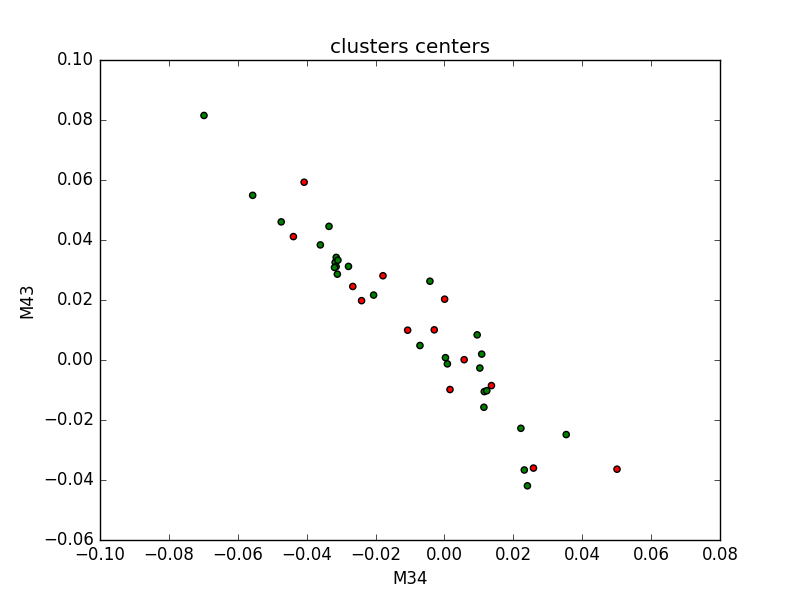
\includegraphics[width=10cm]{PCA_0.png}
\end{figure}
\begin{figure}
  \caption{centre des clusters après transformation}
  \centering
  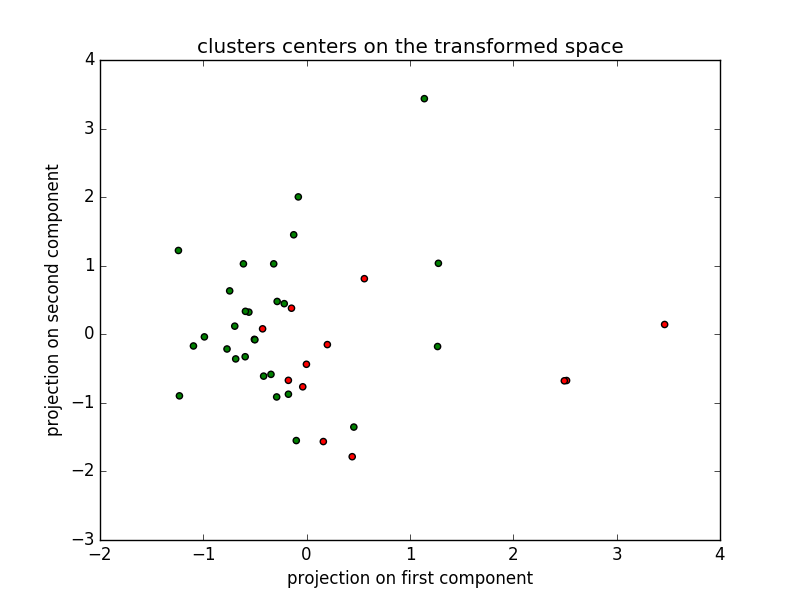
\includegraphics[width=10cm]{PCA_1.png}
\end{figure}
\begin{figure}
  \caption{Part de variance expliquée}
  \centering
  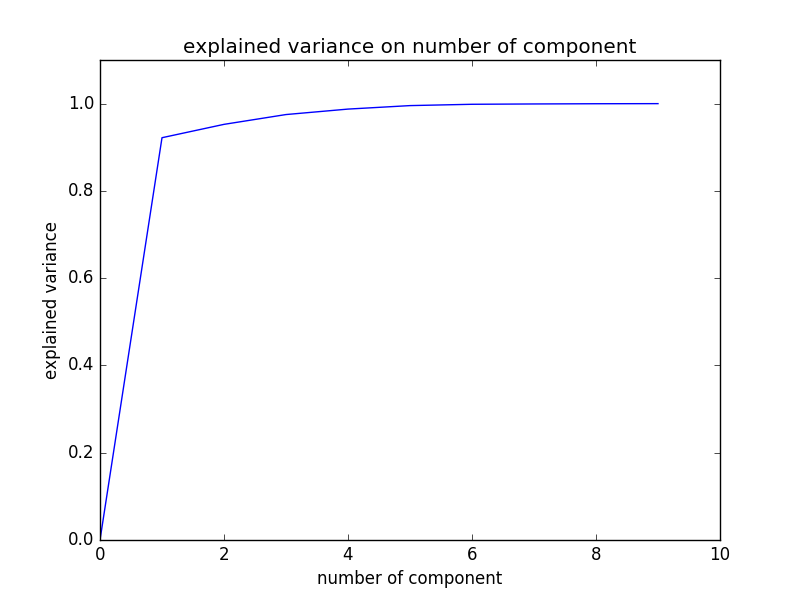
\includegraphics[width=10cm]{PCA_3.png}
\end{figure}
\begin{figure}
  \caption{analyse de la composante principale}
  \centering
  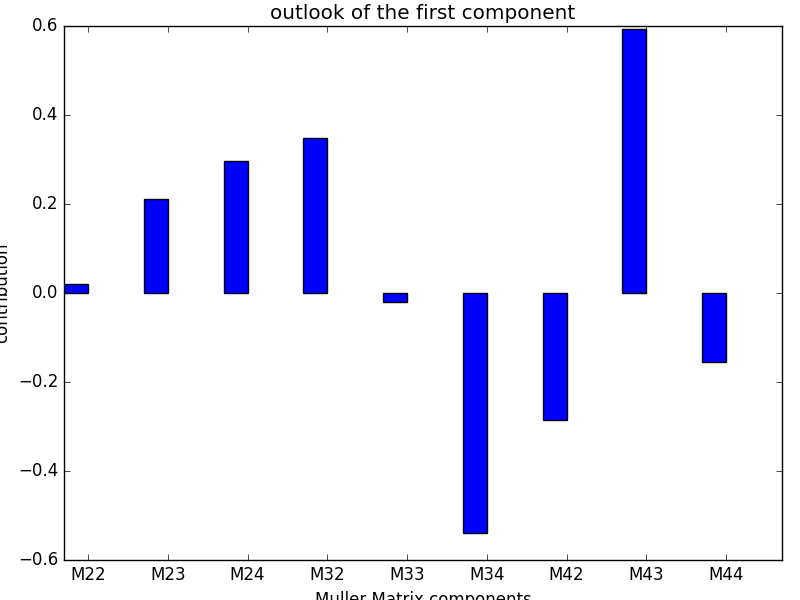
\includegraphics[width=10cm]{PCA_2.png}
\end{figure}

\paragraph{résultats}
La réduction de dimension par PCA semble efficace. La composante principale explique 90\% de la variance (fig 2.3). 
De l'analyse de la première composante (fig 2.4) ressortent deux effets principaux :
- La petite contribution des éléments diagonaux de la matrice de Müller
- Le rôle prépondérant de M34 et M43

On remarque une certaine anti-corrélation des éléments de la matrice de Müller. Le poids de M43 est proche de l'opposé de celui de M34. Le poids de M42 est également proche de l'opposé de celui de M24. Cette observation n'est par contre pas vérifiée pour M23 et M32 qui semblent corrélés.
\paragraph{conclusion}
La PCA effectuée sur les centres des clusters valident certaines hypothèses, comme le faible rôle des éléments diagonaux ou le rôle important des éléments M34 et M43.

Par contre, la projection de la PCA en 2 dimensions ne nous permet pas de séparer les données de manière suffisantes pour être capable de distinguer des zones clairement différentes entre les clusters sains et les clusters malades. (fig 2.2)


\section{Méthode de classification}

\subsection{Arbre décisionnel et Random Forest}
\subparagraph{Arbre décisionnel} 
\index{Arbre de décision}
L'arbre décisionnel est une méthode de classification très classique, qui donne souvent de bons résultats. L'idée est trouver un hyperplan qui sépare au mieux les données (parfois très simple, sur une variable uniquement) et de recommencer cela sur les deux sous-ensembles de données ainsi créés. On isole ainsi les zones où les points sont similaires, et l'on peut ainsi prédire le diagnostic d'un pixel, les hyperplans permettant de construire un arbre de décision.
\subparagraph{Random Forest}
\index{Arbre de décision}
La Random Forest ou forêt d'arbre, est juste un ensemble d'arbres de décision. Les données sont divisées aléatoirement, puis l'on associe à chaque sous-ensemble un arbre de décision. Le résultat de la prédiction se fait par vote, chaque arbre donne sa prédiction, la prédiction majoritaire l'emporte.
\paragraph{Prétraitement utilisé}
Nous avons commencé à apprendre sur toutes les données. Au début, nous avions uniquement les pixels, sans les images associés, puis pour préciser les résultats et limiter le sur-apprentissage, nous les avons classés par image. Nous avons appris au début sur tous les paramètres de la matrice de Müller, puis uniquement sur les 6 éléments significatifs.
\paragraph{Résultats}
L'apprentissage sur les 16 éléments de la matrice de Müller a résulté dans fort sur-apprentissage : l'arbre de décision réussissait à retrouver l'image de provenance, la forte corrélation entre image et diagnostic ne nous permet donc pas d'aller plus loin. L'apprentissage sur 16 images et le test sur la 17éme a permis de dévoiler ce sur-apprentissage, avec des performances renversées et aléatoires. Sur la figure qui suit on peut voir des résultats très élevés (de l'ordre de 95\%) qui témoignent plus d'un sur-apprentissage que d'un réel résultat. En effet, lorsque les ensembles de test et d'apprentissage sont choisis sur des images différentes, les résultats sont beaucoup plus mitigés (autour de 40\%). La restriction à 6 éléments de la matrice n'améliore pas la performance. 
\begin{figure}[htbp]
  \caption{résultats de la Random Forest (pixels mélangés)}
  \centering
  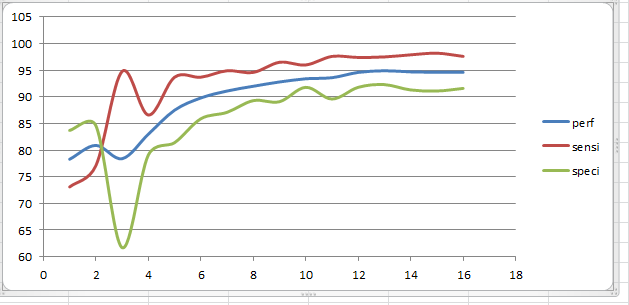
\includegraphics[width=10cm]{RandomForestPerf.png}
\end{figure}
\paragraph{Explication}
Le faible nombre d'images à diagnostic non uniforme conduit l'algorithme à déterminer l'image d’origine puis d’en déduire le diagnostic, les différences entre les images étant plus importantes que les différences de diagnostic. L'apprentissage est biaisé. 
\paragraph{Piste d'amélioration}
Pour résoudre ce problème, il faudrait avoir accès à des images au diagnostic varié, images sur lesquelles un réel apprentissage est possible. N’ayant pas accès à ces images, nous avons décidé de changer de méthode d'apprentissage et de pousser plus loin la compréhension que l'on avait des données.


\subsection{K plus proches voisins}
La méthode des k plus proches voisins ou KNN (K-nearest neighbors) consiste à essayer de prédire l’état d'un nouveau point en se basant sur l'état de ses voisins les plus proches, éventuellement en affectant un poids plus important aux voisins les plus proches. Cette méthode a l'avantage de pouvoir classer les données selon des schémas non linéaires. Par contre, cette méthode est très sensible à la dimension. 
\paragraph{Prétraitement utilisé}
Nous avons testé la méthode des KNN sur les centres des clusters pour plusieurs raisons :

- A chaque classification, l'algorithme doit recalculer l'ensemble des distances avec tout l’échantillon d'apprentissage. Il y a donc une nécessité de réduire le nombre de données en entrée sur lesquels on calcule les distances.

- De plus, chaque cluster regroupe un ensemble de points très proches les uns des autres. Ainsi, en prenant tous les éléments, les plus proches voisins d'un certain point auraient souvent tous appartenu au même cluster, ce qui rend l'information extraite redondante. Cela serait revenu à utiliser l'algorithme avec 1 seul voisin. 
\paragraph{Résultats}
Les résultats présentés ci-dessous correspondent aux taux de bonne prédiction en prenant une image de test et en cherchant les k plus proches voisins sur les 16 autres. Chaque cluster est représenté par un vecteur comprenant les éléments suivants de la matrice de Müller : ['M23', 'M24', 'M32', 'M34', 'M42', 'M43'].
\subparagraph{}
\begin{center}
\begin{tabular}{|c|c|}  
  \hline
  Échantillon de test & taux de bon résultat \\
  \hline
  1 & 100\%\\
  2 & 0\%\\
  3 & 100\%\\
  4 & 100\%\\
  5 & 0\%\\
  6  & 100\%\\
  7 & 33\%\\  
  8 & 50\%\\
  9 & 66\%\\
  10 & 100\%\\
  11 & 100\%\\
  12 & 100\%\\
  13 & 100\%\\
  14 & 75\%\\
  15 & 66\%\\
  16 & 75\%\\
  17 & 100\%\\ 
  \hline
\end{tabular}
\end{center}

En utilisant les 9 éléments de la matrice de Müller Mij avec i et j différents de 1, on obtient un taux moyen de 65\%
\paragraph{Conclusion}
Les résultats donnés par les KNN ne sont pas très bon. En testant cette méthode sur l’ensemble des points (et non pas seulement les centres des clusters, on obtient un taux de précision moyen de 66\%, ce qui confirme notre intuition qu’il suffisait de tester la méthode sur les centres des clusters.
Pour être plus efficace, il faudrait extraire les bons paramètres (feature selection), voire transformer les points dans un espace plus adapté (par exemple en prenant en compte leur norme), et réduire la dimension du problème. Autrement dit, il faudrait mieux comprendre ce qui discrimine les données pour utiliser cette méthode. Elle pourrait être utilisée en complément d’autres méthodes, pour booster les résultats.

\subsection{SVM}
\index{SVM}
Les Machines à Vecteurs Support ou SVM (Support Vector Machine) sont des classifieurs qui cherchent à séparer linéairement deux ensembles de points dans un certain espace, en maximisant la marge entre ces deux sets de points. Par défaut (avec un noyau linéaire), la séparation est donc nécessairement linéaire. Cependant, en transformant nos données pour les plonger dans un autre espace, souvent de dimension supérieure, on peut générer un modèle de capacité supérieure et fortement non linéaire. C'est ce qu'on appelle le Kernel trick\index{Kernel trick}

\paragraph{Prétraitement utilisé}
Les SVM sont efficaces lorsque le nombre de paramètres est très inférieur au nombre de données. On applique donc cette méthode aux points directement, et non pas aux centres des clusters.

\paragraph{Résultats}

\begin{figure}[H]
  \centering  
  \caption{Résultats de la méthode SVM: proportion de bonnes prédictions et nombre de pixels dans l'ensemble de test, pour chaque image.}
  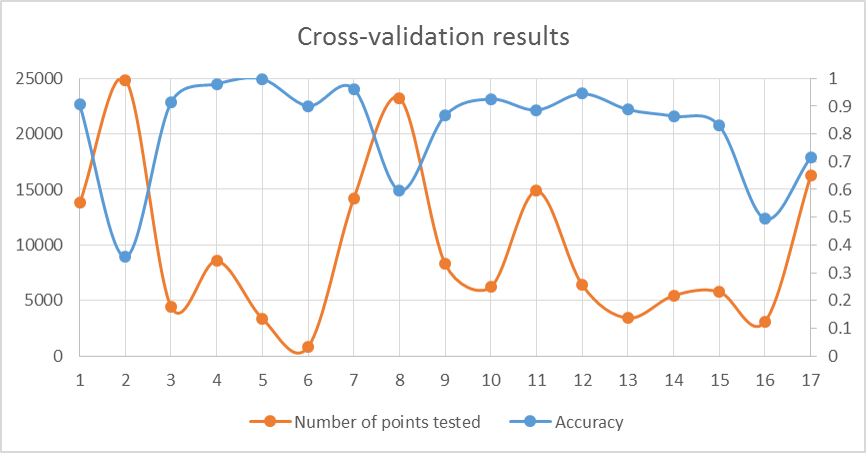
\includegraphics[width=10cm]{SVM_CV.png}
\end{figure}

\paragraph{Explication et piste d'amélioration}
Le problème du Kernel trick\index{Kernel trick} est qu'il nécessite d'avoir une idée a priori du type de fonction que l'on cherche à estimer pour pouvoir utiliser un noyau adéquat. Ce n'est ici pas le cas, on ne sait pas a priori quel pourrait être le type de fonction permettant de distinguer un pixel sain d'un pixel malade.

Pour résoudre ce problème, il faudrait "apprendre la fonction noyau". C'est en quelque sorte le rôle des neural networks.\index{Neural networks}. On peut voir les n-1 couches du réseau de neurones comme étant la fonction du noyau et la dernière comme une séparation linéaire sur les données plongées dans ce nouvel espace.

\subsection{Réseaux de Neurones}

Comme évoqué précédemment, les Neural Networks sont une piste naturels à explorer lorsque l’on n’a pas d'idée a priori de la forme du "bon" noyau à utiliser dans les SVMs. Un réseau de neurones consiste en une succession de couche de neurones. La première couche de neurones correspond aux données d'entrée et la dernière à la prédiction souhaitée. L'avantage principal des réseaux neuronaux est d'être capable, dès lors que le réseau a plus de deux couches, d'apprendre des fonctions fortement non linéaires sans a priori sur leur forme. Nous avons utilisé une pénalisation linéaire de la norme des poids. 

La fonction de coup qu'on cherche à minimiser est la suivante :
\begin{equation}
\begin{split} 
J(\theta)= \frac{1}{m} \sum_{i=1}^m \sum_{k=1}^K -y_k^{(i)} log((h_{\theta}(x^{(i)}))_k) - (1 - y_k^{(i)}log(1 - h_{\theta}(x^{(i)}))_k))\\
 + \frac{\lambda}{2m}[\sum_{j=1}^7\sum_{k=1}^{50}(\theta_{j,k}^{(1)})^2 + \sum_{j=1}^{50}\sum_{k=1}^{50}(\theta_{j,k}^{(2)})^2 + \sum_{j=1}^{50}\sum_{k=1}^2(\theta_{j,k}^{(3)})^2]
\end{split}
\end{equation} 

+\begin{figure}[H]
 +  \centering  
 +  \caption{Schéma éxplitaif représetant un réseau de neuronnes}
 +  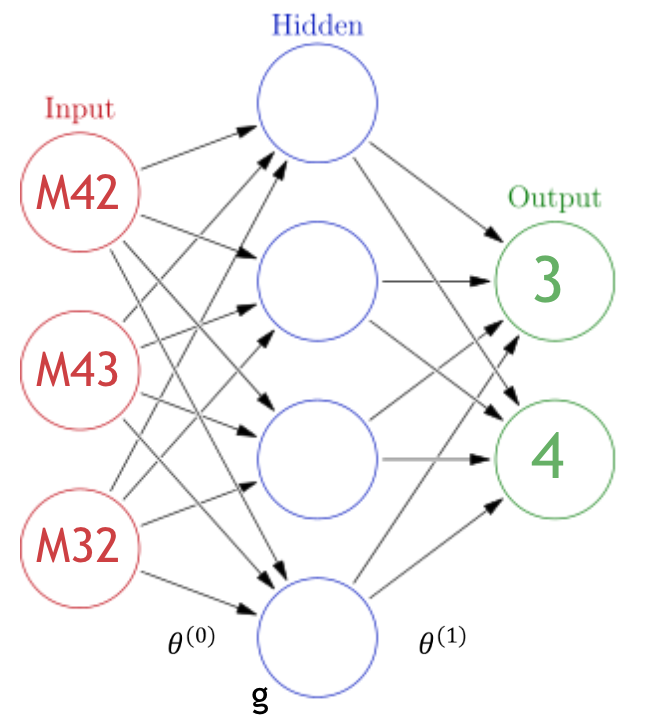
\includegraphics[width=7cm]{nn_explanation.png}
 +\end{figure}

\paragraph{prétraitement}
Le prétraitement correspond ici aux choix des données à mettre dans la première couche. Nous avons utilisé un maximum d'input dans un premier temps. En étudiant les premiers résultats, nous avons pu estimer quels imputs avaient le plus d’impact sur la décision finale. Après plusieurs itérations et tests, nous avons conclus que les éléments les plus importants étaient les suivants :

\begin{itemize}

    \item Les éléments de la matrice de Müller : M32, M43, M33, M42

    \item La norme 1 de la matrice de Müller 
    
    \item La norme 2 de la matrice de Müller 

    \item La norme infinie de la matrice de Müller  

\end{itemize}

Notons que le choix de ces paramètres n’est pas nécessairement optimal. En effet, en réduisant le nombre de paramètres d’entrée, on simplifie le problème, ce qui peut en contrepartie améliorer les résultats de prédiction. Il faudrait tester différentes combinaisons de paramètres et laisser l’algorithme tourner plusieurs heures pour mieux sélectionner les différents paramètres.

\begin{figure}[htbp]
  \caption{Poids des inputs}
  \centering
  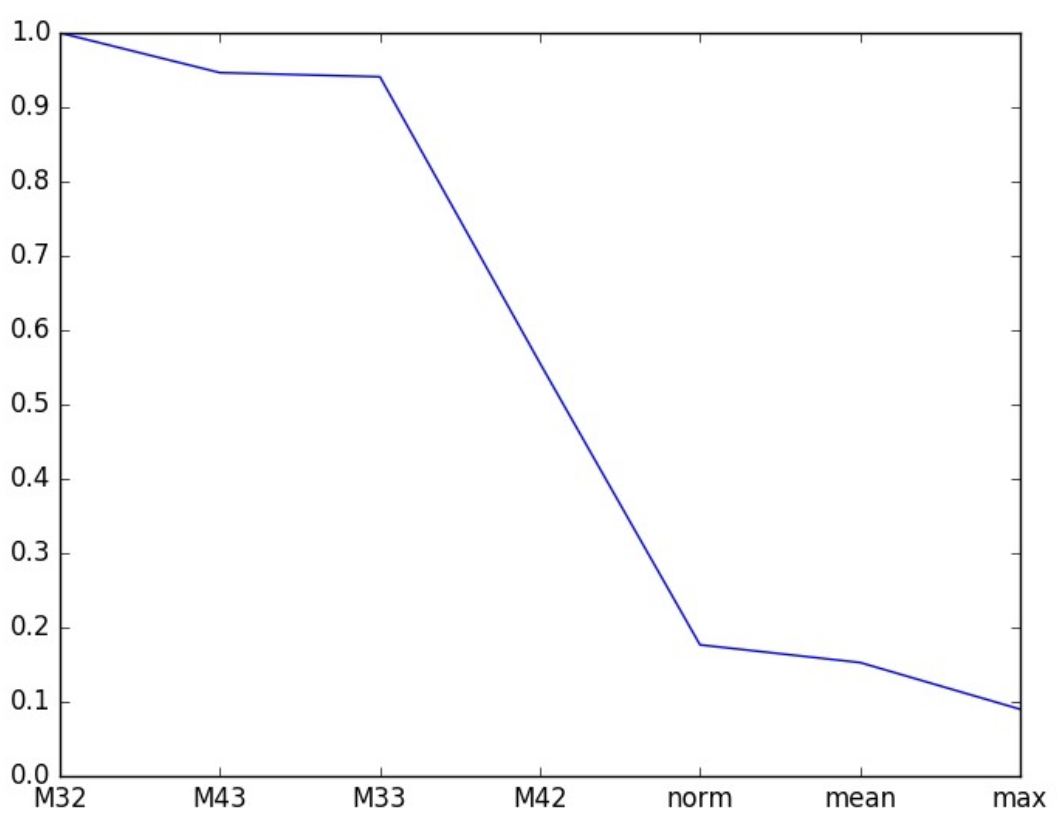
\includegraphics[width=10cm]{input_weight_nn.png}
\end{figure}

\paragraph{Résultats}
Les résultats présentés ici sont obtenus avec un réseau de quatre couches : [7, 50, 50, 2], une constante de pénalisation de 0.5, et 200 itérations de la fonction de minimisation.
On obtient un taux de bonnes prédictions moyen de 80\% en effectuant une validation croisée avec un apprentissage sur 16 images et test sur la 17ème. 

Les résultats seraient sûrement améliorés en augmentant le nombre d'itération et en s'appuyant sur un set de donnée plus large. En l'état, les résultats sont comparables à ceux donnés par les SVMs.
\begin{figure}[htbp]
  \caption{Résultats de la classification avec des neural networks}
  \centering
  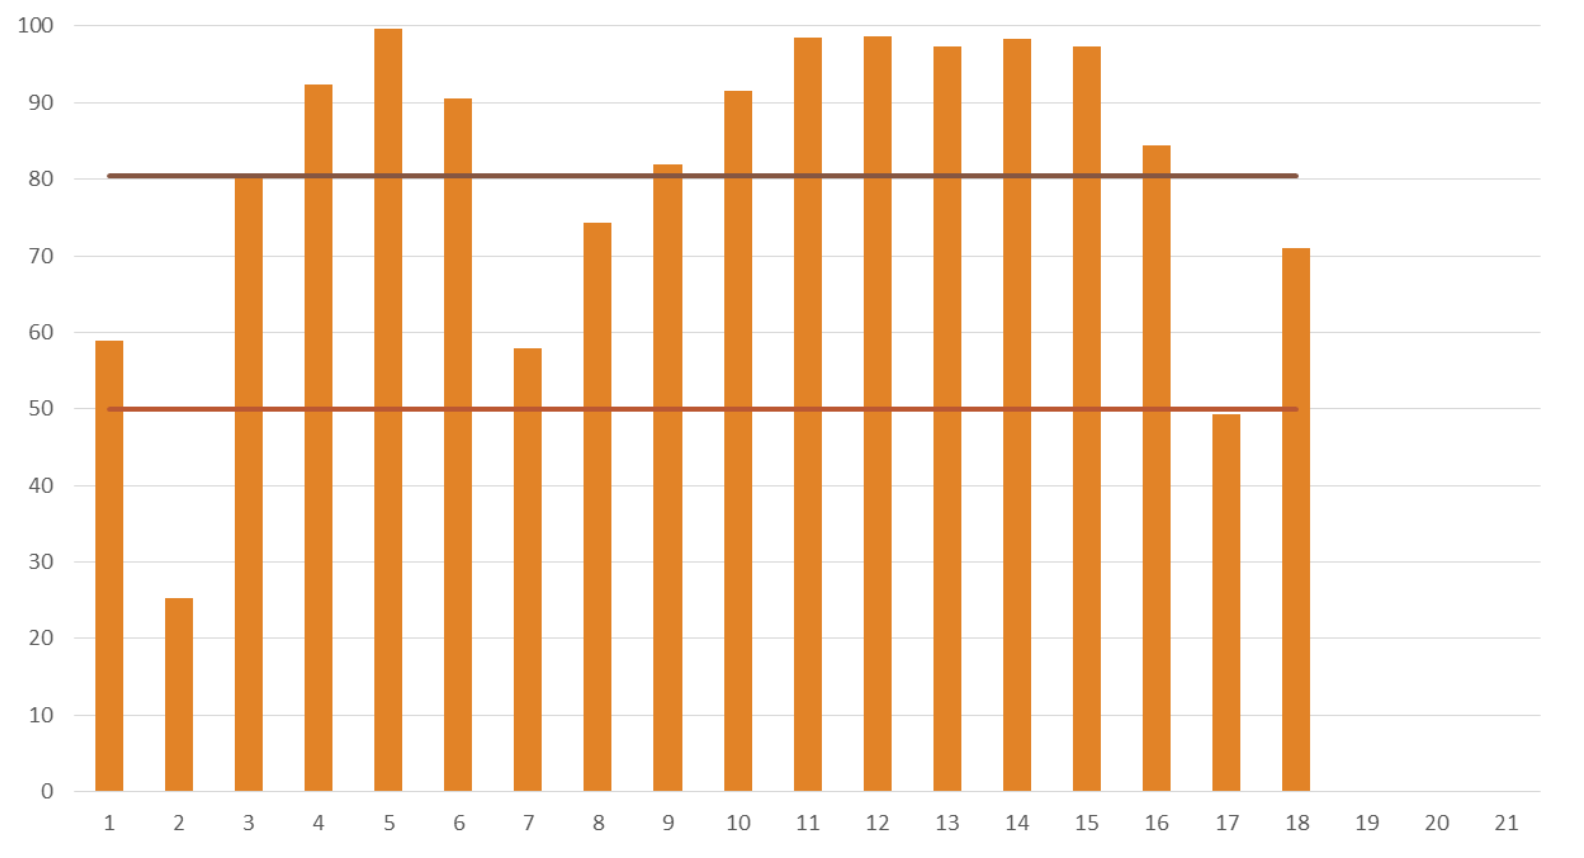
\includegraphics[width=10cm]{nn_results.png}
\end{figure}

\section{Comparaison des méthodes de classifications}

\begin{figure}[htbp]
  \caption{Comparaison des taux de bonne prédiction des différentes méthodes de classification testées.}
  \centering
  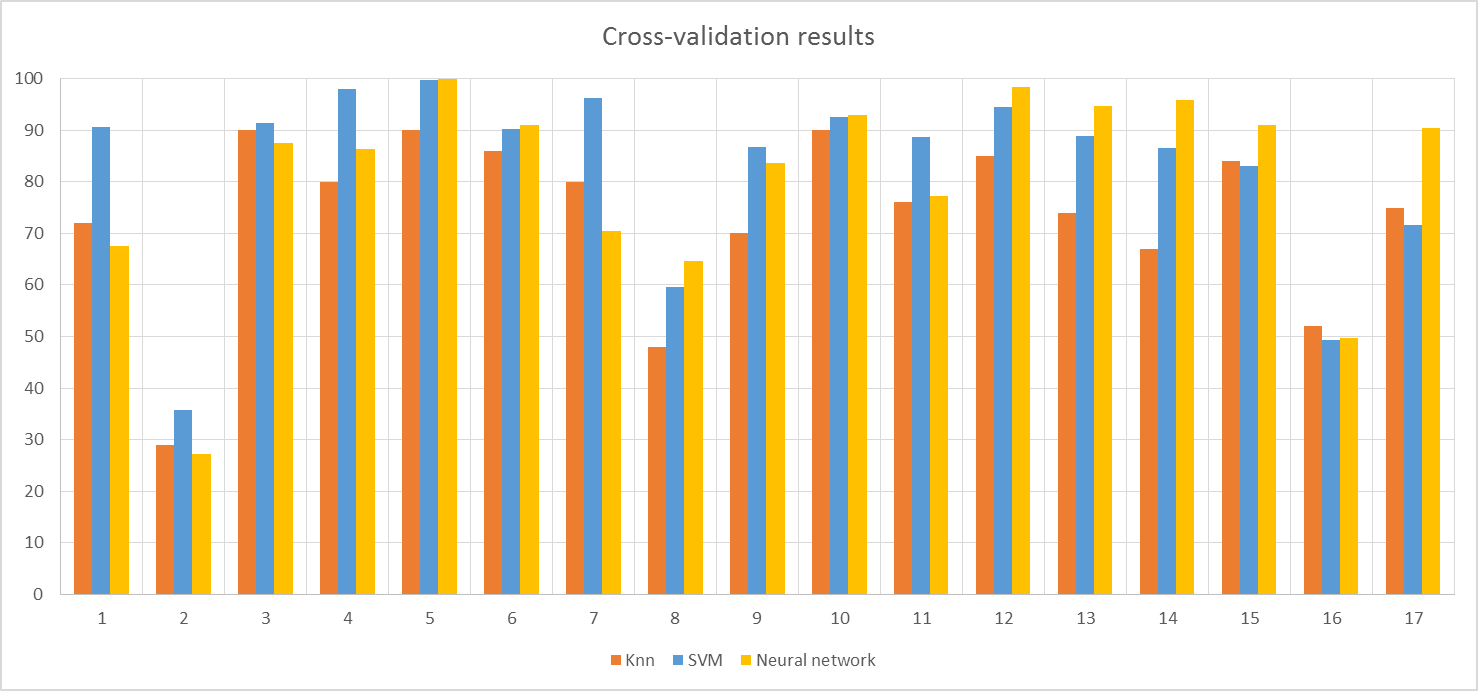
\includegraphics[width=10cm]{Compared_CV.png}
\end{figure}

\begin{center}
Moyenne des taux de précision\\

\begin{tabular}{|c|c|c|}  
  \hline
  Méthode & Moyenne simple & Moyenne pondérée\\
  \hline
  KNN & 73.41 & 65.75\\
  Neural Network & 80.49 & 71.70\\  
  SVM & 82.56 & 75.65\\
  \hline
\end{tabular}
\end{center}

Ce tableau présente les taux de précision moyens des méthodes précédentes, soit en moyennant sur chaque image, soit en pondérant les résultats par le nombre de pixels de l'image (ainsi, chaque pixel intervient 1 fois dans le calcul final, selon sa classification à partir de 16 autres images).

La méthode Knn semble avoir de moins bons résultats que les méthodes SVM et Neural network. 

Par ailleurs, on remarque que les images ayant beaucoup de pixels (les images 2 et 8 représentent 30\% des pixels) ont des moins bons taux de prédiction, ce qui pourrait indiquer que nous n'avons pas atteint le seuil de données critiques nécessaires à des résultats optimaux. En effet, en augmentant le nombre d’itérations de la fonction de minimisation pour la validation croisée de l’image 2, de 200 à 5000, le taux de précision croît de 32 à 67\%. En contrepartie, le temps de calcul passe de 4 minutes à plus d’une heure et demie. Ceci confirme que l’on peut fortement améliorer les résultats, simplement en augmentant le temps de calcul, pour garantir un taux de précision plus élevé.
Avec quelques images supplémentaires, on pourrait espérer garantir un taux de précision d'au moins 80\% à 90\% avec cette méthode. On pourrait également combiner les différentes méthodes précédentes : si elles ne se trompent pas simultanément, on pourrait ainsi booster les résultats de prédiction.
Notons enfin que l'image 16 a également un taux de précision très faible, en dépit de son petit nombre de points. C'est la seule image ayant à la fois des zones saines et malades, il semble donc que les méthodes aient tendance à prédire le même diagnostic pour les pixels d'une même image.
Dans les circonstances actuelles, certaines images ont des résultats très inférieurs à cette valeur moyenne, voire en-deçà de 50\%: ces méthodes ne sont donc pas assez fiable pour permettre de bien classifier les données.


\chapter*{Conclusion}
Ce pojet de Big Data nous a permis de mettre en place un classifieur sur des images, plus précisément des pixels, puisque nous nous intéressons à une propriété locale de l'image. La compréhension et l'analyse des données nous ont pris beaucoup plus de temps que prévu, en particulier à cause de la répartition et du faible nombre de données. Néanmoins, les données étaient de très bonne qualité et facilement exploitable, et nous avons réussi, après de nombreuses tentatives, à trouver des modèles qui arrivent à apprendre sur les données sans sur-apprentissage. La SVM et le réseau de neurones ont de bons résultats, avec des taux de prédiction peuvent être exploitable. Pour aller plus loin, en plus de la combinaison des méthodes d’apprentissage et le réglage optimal de leurs paramètres, il faudrait analyser les images après prédiction pour améliorer les résultats par la cohérence spatiale des prédictions. On pourrait également étudier les pistes de prétraitement qui permettraient des nettoyer les données et de prendre en compte la configuration de l'appareil au moment de la mesure. L’entraînement de ce classifieur sur un gros réseau de neurones, avec toutes les données disponibles, permettrait d'atteindre des taux de prédiction très compétitifs. Pour compléter l'analyse et pouvoir l'utiliser en médecine, il faudra aussi analyser la spécificité et la sensibilité afin de jouer sur les paramètres, car l’erreur ne sera pas permise.

\tableofcontents
\listoffigures
\end{document}
